\documentclass[]{report}
\usepackage{hyperref}
\usepackage{amsmath}
\usepackage{graphicx}
\usepackage[]{mcode}

\hypersetup{colorlinks=true, linkcolor=black, urlcolor=blue}
% Title Page
\title{Project: Image Analysis 2015/2016\\Anomaly Detection for Crop Monitoring}

\author{Stefano Cerri 849945}


\begin{document}
\maketitle
\tableofcontents
\listoffigures

\chapter{Scope}

\section{Problem}

One of the most important tasks to be addressed in intelligent farms is the crop monitoring. Computer Vision and Machine Learning algorithms are typically combined to analyze and classify images acquired by autonomous robots that monitor the growth of crops, and in particular, to discriminate crops (i.e. the good plants) from weeds (any undesirable or unwanted plant growing wild, especially those that takes food or nourishment from crops). Crop/weed discrimination of often tacked as an image-classification problem.


\section{Dataset}

The dataset used in this project is the CWFID dataset\footnote{https://github.com/cwfid/dataset}. It comprises field images, vegetation segmentation masks and crop/weed plant type annotations. The paper\footnote{see Appendix$\rightarrow  $Reference document} provides details, e.g. on the field setting, acquisition conditions, image and ground truth data format.
All images were acquired with the autonomous field robot Bonirob in an organic carrot farm while the carrot plants were in early true leaf growth stage.

\section{Assignment}

The assignment is to create a Convolutional Neural Network that classificates the images in crop,weed or ground. 

\chapter{Extract patches from the dataset}

This work was done by two collegues,Jorge Carpio Lopez de Castro and  Andrea Luigi Edoardo Caielli, that work on the same project. 
Here is the code:

\begin{lstlisting}

% IMAGE ANALYSIS - PROJECT 2015/2016
%
% Script for extracting from CWFID N random image patches centered
% on pixels which are marked in the ground truth as a given class.
% Patches can be extracted for testing or training. Training paches are
% extracted from the first 40 imgs. of the dataset. Testing patches come
% from the last 20.
%
% Requires the CWFID dataset to be downloaded and placed in the workspace.

warning('off', 'Images:initSize:adjustingMag');
close all, clear all
clc

%% Configurable parameters

N = 1000;           % Number of patches for each class.
psz = 51;           % Size of the sides of the patch [pixels].

option = 1;         % 1 for training patches (extracted from first 40 images),
                        % 0 for test patches (extracted from last 20).
                        
se = strel('disk', 8);  % Shape for the erosion of the center pixels for the patches.

%% Code

np = N * ones(1,3); % Overall number of remaining patches to be extracted 
                        % for each class. One counter is not sufficient since
                        % not all images have information for all three classes.
classes = [1 1 1];      % Class selector for patch extraction

if option == 0      % Extracting set of patches for training
   n_im = 40;                   % Number of images of the dataset for trai.
   bpath = 'patches\training\'; % Base path for folder
elseif option == 1  % Extracting set of patches for testing
   n_im = 20;                   % Number of images of the dataset for test.
   bpath = 'patches\testing\';  % Base path for folder
else
    return;
end

mkdir(bpath);       % Create directories
mkdir(bpath,'weed'); 
mkdir(bpath,'crop'); 
mkdir(bpath,'ground');

fs = ['%0' num2str(floor(log10(N))+1) 'd']; % Format string used for output
disp('Begin extracting random 51x51 patch images:')
str = [fs '\t' fs '\t' fs];
str2 = ['Remaining patches:\n\tweed\tcrop\tground\n\t' str];
fprintf(str2, np(1), np(2), np(3))

while(sum(np))  % while there are remaining patches 
    rand_im_ix = randi(n_im,1,max(np));  
                                        % Image numbers to get patches from.
                                        % This maintains randomness
                                        % minimizing image reads.
                                       
    imgs = zeros(1,n_im);               % Number of patches / each image in
                                            % rand_im_ix
    for n = 1:max(np)
        imgs(rand_im_ix(n)) = imgs(rand_im_ix(n)) + 1;
    end

    for im = find(imgs)
        ann_path = strcat( 'dataset-1.0\annotations\', sprintf('%03d',im + 40*option),...
                '_annotation.png');     % Path for annotation file
            
        img_path = strcat( 'dataset-1.0\images\', sprintf('%03d',im + 40*option),...
                '_image.png');          % Path for image file

        A = imread( ann_path, 'png');   % Read annotation mask
        I = imread( img_path, 'png');   % Read corresponding image   

        for n = 1:imgs(im)     % Each iteration finds a new rand. 51x51 patch

            c = 1:3;
            classes = ~~np;    % Flags indicating remaining patches != 0
            for c = c(classes) % Main loop for each class (weed, crop, ground) 
                
                switch c      % Perform class-oriented operations
                    case 1
                        IMask = im2bw(A(:,:,1));    % Binary mask (weed)
                        filename = [bpath 'weed\' sprintf(fs,np(c)) '_weed.png'];
                    case 2
                        IMask = im2bw(A(:,:,2));    % Binary mask (crop)
                        filename = [bpath 'crop\' sprintf(fs,np(c)) '_crop.png'];
                    otherwise                       % Binary mask (ground)
                        IMask = ~(im2bw(A(:,:,1)) | im2bw(A(:,:,2)));
                        filename = [bpath 'ground\' sprintf(fs,np(c)) '_ground.png'];
                end
                
                Centers = IMask(ceil(psz/2):end-floor(psz/2),...
                          ceil(psz/2):end-floor(psz/2)); % Possible center points
                Centers = imerode(Centers,se);  % Perform erosion
                [y, x] = find(Centers);  % x,y: coordinate arrays for nonzero elts.

                if ~(isempty(y) || isempty(x)) % Then this image has 
                                               % annotations for this class 
               
                    np(c) = np(c) - 1;    % Decrement remaining patches
                    p = randi(length(y)); % Index for (random again) center pix
                    P = I(y(p):y(p)+psz-1, x(p):x(p)+psz-1, :); % Patch
                    imwrite(P, filename, 'png');
                end  
            end
            for i = 1:2+3*floor(log10(N)+1), fprintf('\b'); end     % Super stylish output
            fprintf(str, np(1), np(2), np(3))
        end
    end
end
fprintf('\nDone!!\n')

\end{lstlisting}

This script creates a dataset of 1000 patches with dimension $ 51\times51\times3 $ for each class both for training and for testing. Later I splitted the testing dataset in two parts:
\begin{itemize}
\item first half of the patches for validation
\item second half of patches for testing

\end{itemize}   

\chapter{Training the network}

\section{MatConvNet library}

In order to perform the given assignment I donloaded and installed MatConvNet library\footnote{http://www.vlfeat.org/matconvnet/}. Note that in order to use some functionalities of the library, such as using GPU acceleration, it has some requirements\footnote{http://www.vlfeat.org/matconvnet/gpu/}.
If you don't know what a convolutional neural network is, there is also a manual\footnote{http://www.vlfeat.org/matconvnet/matconvnet-manual.pdf} that explains all the blocks of a CNN both from the "mathematical" and "code function" view.  

\section{Build the architecture of the network}

\subsection{Typical layer of a CNN}

The typical layer of a Convolutional Neural Network are:

\begin{itemize}

\item \textbf{Convolutional layer}:it is the core building block of a Convolutional Network, and its output volume can be interpreted as holding neurons arranged in a 3D volume.The CONV layer's parameters consist of a set of learnable filters. Every filter is small spatially (along width and height), but extends through the full depth of the input volume. During the forward pass, we slide (more precisely, convolve) each filter across the width and height of the input volume, producing a 2-dimensional activation map of that filter. As we slide the filter, across the input, we are computing the dot product between the entries of the filter and the input. Intuitively, the network will learn filters that activate when they see some specific type of feature at some spatial position in the input. Stacking these activation maps for all filters along the depth dimension forms the full output volume. Every entry in the output volume can thus also be interpreted as an output of a neuron that looks at only a small region in the input and shares parameters with neurons in the same activation map (since these numbers all result from applying the same filter).Three hyperparameters control the size of the output volume: the \textbf{depth}, \textbf{stride} and \textbf{zero-padding}

\item \textbf{Pooling Layer}:it is common to periodically insert a Pooling layer in-between successive Conv layers in a ConvNet architecture. Its function is to progressively reduce the spatial size of the representation to reduce the amount of parameters and computation in the network, and hence to also control overfitting. The Pooling Layer operates independently on every depth slice of the input and resizes it spatially, using the MAX operation. The most common form is a pooling layer with filters of size 2x2 applied with a stride of 2 downsamples every depth slice in the input by 2 along both width and height, discarding 75\% of the activations. Every MAX operation would in this case be taking a max over 4 numbers (little 2x2 region in some depth slice). The depth dimension remains unchanged

\item \textbf{Fully-connected layer}:neurons in a fully connected layer have full connections to all activations in the previous layer. Their activations can hence be computed with a matrix multiplication followed by a bias offset.In other libraries,fully connected blocks or layers are linear functions where each output dimension depends on all the input dimensions.MatConvNet does not distinguish between fully connected layers and convolutional blocks

\item \textbf{ReLu}:the rectified linear unit will apply an elementwise activation function, such as the $ f(x) = max(0,x) $ thresholding at zero. This leaves the size of the volume unchanged 

\item \textbf{SoftMax}: Soft Max is a loss functionakes the score compete through the normalization
factor.Softmax can be seen as the combination of an activation function
(exponential) and a normalization operator

\end{itemize}


\subsection{Typical architecture}

The most common form of a ConvNet architecture stacks a few CONV-RELU layers, follows them with POOL layers, and repeats this pattern until the image has been merged spatially to a small size. At some point, it is common to transition to fully-connected layers. The last fully-connected layer holds the output, such as the class scores. In other words, the most common ConvNet architecture follows the pattern:

$INPUT\rightarrow [[CONV\rightarrow RELU]*N\rightarrow POOL?]*M\rightarrow[FC\rightarrow RELU]*K\rightarrow FC \rightarrow LOSS $

where the $ * $ indicates repetition, and the POOL? indicates an optional pooling layer. Moreover, $ N>=0 $ (and usually $ N<=3 $), $M >= 0$,$ K >= 0$ (and usually $ K < 3$).

\subsection{Selected architectures}

I selected different network architectures for comparing it, after the training, with the testing set. The architectures are:

\begin{enumerate}

\item $ INPUT \rightarrow [CONV \rightarrow RELU \rightarrow POOL]*2 \rightarrow FC \rightarrow RELU \rightarrow FC \rightarrow LOSS $ 

\item $ INPUT \rightarrow [CONV \rightarrow RELU \rightarrow POOL]*3 \rightarrow FC \rightarrow LOSS $ 

\item $ INPUT \rightarrow [CONV \rightarrow RELU \rightarrow POOL]*4 \rightarrow FC \rightarrow LOSS $ 

\item $ INPUT \rightarrow [CONV \rightarrow RELU \rightarrow POOL]*3 \rightarrow FC \rightarrow LOSS $ 

\item $ INPUT \rightarrow [CONV \rightarrow RELU \rightarrow POOL]*3 \rightarrow FC \rightarrow RELU \rightarrow FC \rightarrow LOSS $ 

\item $ INPUT \rightarrow [CONV \rightarrow RELU \rightarrow POOL]*3 \rightarrow [FC \rightarrow RELU]*2 \rightarrow FC \rightarrow LOSS $ 

\end{enumerate}

Here is the code of the first architecture. The other architectures are in other matlab file, structured as cnn\textunderscore cwfid\textunderscore init\textunderscore number\textunderscore of\textunderscore the\textunderscore network.

\begin{lstlisting}
%Function that creates the convolutional neural network
function net = cnn_cwfid_init_1(varargin)

%decide if you want to use batch normalization
opts.batchNormalization = true ;
%decide if you want to use simplenn or dagnn
opts.networkType = 'simplenn' ;
opts = vl_argparse(opts, varargin) ;

rng('default');
rng(0) ;

%create the network layers
f=1/100 ;
net.layers = {} ;
net.layers{end+1} = struct('name', 'convolution1',...
                           'type', 'conv', ...
                           'weights', {{f*randn(9,9,3,20, 'single'), zeros(1, 20, 'single')}}, ...
                           'stride', 1, ...
                           'pad', 0) ;
net.layers{end+1} = struct('name','relu1','type','relu');                         
net.layers{end+1} = struct('name', 'pooling1',...
                           'type', 'pool', ...
                           'method', 'max', ...
                           'pool', [2 2], ...
                           'stride', 2, ...
                           'pad', 0) ;
net.layers{end+1} = struct('name', 'convolution2',...
                           'type', 'conv', ...
                           'weights', {{f*randn(7,7,20,40, 'single'),zeros(1,40,'single')}}, ...
                           'stride', 1, ...
                           'pad', 0) ;
net.layers{end+1} = struct('name','relu1','type','relu');                           
net.layers{end+1} = struct('name', 'pooling2',...
                           'type', 'pool', ...
                           'method', 'max', ...
                           'pool', [2 2], ...
                           'stride', 2, ...
                           'pad', 0) ;                          
net.layers{end+1} = struct('name', 'convolution3',...
                           'type', 'conv', ...
                           'weights', {{f*randn(7,7,40,200, 'single'),  zeros(1,200,'single')}}, ...
                           'stride', 1, ...
                           'pad', 0) ;
net.layers{end+1} = struct('name','relu1','type','relu');                            
net.layers{end+1} = struct('name', 'convolution4',...
                           'type', 'conv', ...
                           'weights', {{f*randn(1,1,200,3, 'single'), zeros(1,3,'single')}}, ...
                           'stride', 1, ...
                           'pad', 0) ;
net.layers{end+1} = struct('name', 'loss','type', 'softmaxloss') ;

% optionally switch to batch normalization
if opts.batchNormalization
  net = insertBnorm(net, 1) ;
  net = insertBnorm(net, 5) ;
  net = insertBnorm(net, 9) ;
end

% Meta parameters
net.meta.inputSize = [51 51 3] ;
net.meta.trainOpts.learningRate = 0.001 ;
net.meta.trainOpts.numEpochs = 30 ;
net.meta.trainOpts.batchSize = 500 ;

% Fill in defaul values
net = vl_simplenn_tidy(net) ;

% Switch to DagNN if requested
switch lower(opts.networkType)
  case 'simplenn'
    % done
  case 'dagnn'
    net = dagnn.DagNN.fromSimpleNN(net, 'canonicalNames', true) ;
    net.addLayer('error', dagnn.Loss('loss', 'classerror'), ...
             {'prediction','label'}, 'error') ;
  otherwise
    assert(false) ;
end

%Function that insert batch normalization
% --------------------------------------------------------------------
function net = insertBnorm(net, l)
% --------------------------------------------------------------------
assert(isfield(net.layers{l}, 'weights'));
ndim = size(net.layers{l}.weights{1}, 4);
layer = struct('type', 'bnorm', ...
               'weights', {{ones(ndim, 1, 'single'), zeros(ndim, 1, 'single')}}, ...
               'learningRate', [1 1 0.05], ...
               'weightDecay', [0 0]) ;
net.layers{l}.biases = [] ;
net.layers = horzcat(net.layers(1:l), layer, net.layers(l+1:end)) ;

\end{lstlisting}

\section{Train the network}

In order to train the network I use this code that prepare the dataset, create the network and train it.

\begin{lstlisting}
%This function create the network and train it with the CWFID dataset
function [net, info] = cnn_cwfid(varargin)

%setup MatConvNet
run(fullfile(fileparts(mfilename('fullpath')),...
  '..', '..', 'matlab', 'vl_setupnn.m')) ;

%Uncomment the line below if you want to use GPU
%vl_compilenn('enableGpu', true);

%batch normalization
opts.batchNormalization = true ;
%network type: simplenn or dagnn
opts.networkType = 'simplenn' ;
[opts, varargin] = vl_argparse(opts, varargin) ;

%create the folder (bnorm if opts.batchNormalization = true
sfx = opts.networkType ;
if opts.batchNormalization, sfx = [sfx '-bnorm'] ; end
opts.expDir = fullfile(vl_rootnn, 'data', ['cwfid-baseline' sfx]) ;
[opts, varargin] = vl_argparse(opts, varargin) ;
opts.dataDir = fullfile(vl_rootnn, 'data', 'cwfid') ;
opts.imdbPath = fullfile(opts.expDir, 'imdb.mat');
opts.train = struct() ;
opts = vl_argparse(opts, varargin) ;
if ~isfield(opts.train, 'gpus'), opts.train.gpus = []; end;

% --------------------------------------------------------------------
%                                                         Prepare data
% --------------------------------------------------------------------

%if you want to use a different network change the function name
%e.g. cnn_cwfid_init_1
%if you have already a folder with a trained network, please remove it
%before train
net = cnn_cwfid_init_5('batchNormalization', opts.batchNormalization, ...
                     'networkType', opts.networkType) ;
imdb = getCwfidImdb(opts) ;
mkdir(opts.expDir) ;
save(opts.imdbPath, '-struct', 'imdb') ;


net.meta.classes.name = arrayfun(@(x)sprintf('%d',x),1:3,'UniformOutput',false) ;

% --------------------------------------------------------------------
%                                                                Train
% --------------------------------------------------------------------

%switch to different training type depending the network type is simplenn
%or dagnn
switch opts.networkType
  case 'simplenn', trainfn = @cnn_train ;
  case 'dagnn', trainfn = @cnn_train_dag ;
end

[net, info] = trainfn(net, imdb, getBatch(opts), ...
  'expDir', opts.expDir, ...
  net.meta.trainOpts, ...
  opts.train);

% --------------------------------------------------------------------
function fn = getBatch(opts)
% --------------------------------------------------------------------
switch lower(opts.networkType)
  case 'simplenn'
    fn = @(x,y) getSimpleNNBatch(x,y) ;
  case 'dagnn'
    bopts = struct('numGpus', numel(opts.train.gpus)) ;
    fn = @(x,y) getDagNNBatch(bopts,x,y) ;
end

% --------------------------------------------------------------------
function [images, labels] = getSimpleNNBatch(imdb, batch)
% --------------------------------------------------------------------
images = imdb.images.data(:,:,:,batch) ;
labels = imdb.images.labels(1,batch) ;

% --------------------------------------------------------------------
function inputs = getDagNNBatch(opts, imdb, batch)
% --------------------------------------------------------------------
images = imdb.images.data(:,:,:,batch) ;
labels = imdb.images.labels(1,batch) ;
if opts.numGpus > 0
  images = gpuArray(images) ;
end
inputs = {'input', images, 'label', labels} ;

% --------------------------------------------------------------------
function imdb = getCwfidImdb(opts)
% --------------------------------------------------------------------
% Preapre the imdb structure
cropLabel = 1;
weedLabel = 2;
groundLabel = 3;

trainingDir = fullfile(opts.dataDir,'training');
%only the first half of the testing images are using for validation
validationDir = fullfile(opts.dataDir,'testing');

trainingCropDir = fullfile(trainingDir,'crop');
trainingWeedDir = fullfile(trainingDir,'weed');
trainingGroundDir = fullfile(trainingDir,'ground');

validationCropDir = fullfile(validationDir,'crop');
validationWeedDir = fullfile(validationDir,'weed');
validationGroundDir = fullfile(validationDir,'ground');

%get training crop images and labels
listing = dir(trainingCropDir);
listing=listing(~ismember({listing.name},{'.','..','Thumbs.db'}));
for i=1 : size(listing)
    cropImTraining(:,:,:,i)=imread(fullfile(trainingCropDir,listing(i).name));
    cropLabelTraining(i) = cropLabel;
end

%get training weed images and labels
listing = dir(trainingWeedDir);
listing=listing(~ismember({listing.name},{'.','..','Thumbs.db'}));
for i=1 : size(listing)
    weedImTraining(:,:,:,i)=imread(fullfile(trainingWeedDir,listing(i).name));
    weedLabelTraining(i) = weedLabel;
end

%get training ground images and labels
listing = dir(trainingGroundDir);
listing=listing(~ismember({listing.name},{'.','..','Thumbs.db'}));
for i=1 : size(listing)
    groundImTraining(:,:,:,i)=imread(fullfile(trainingGroundDir,listing(i).name));
    groundLabelTraining(i) = groundLabel;
end

%get validation crop images and labels
listing = dir(validationCropDir);
listing=listing(~ismember({listing.name},{'.','..','Thumbs.db'}));
for i=1 : (size(listing,1) - 500)
    cropImValidation(:,:,:,i)=imread(fullfile(validationCropDir,listing(i).name));
    cropLabelValidation(i) = cropLabel;
end

%get validation weed images and labels
listing = dir(validationWeedDir);
listing=listing(~ismember({listing.name},{'.','..','Thumbs.db'}));
for i=1 : (size(listing,1) - 500)
    weedImValidation(:,:,:,i)=imread(fullfile(validationWeedDir,listing(i).name));
    weedLabelValidation(i) = weedLabel;
end

%get validation ground images and labels
listing = dir(validationGroundDir);
listing=listing(~ismember({listing.name},{'.','..','Thumbs.db'}));
for i=1 : (size(listing,1) - 500)
    groundImValidation(:,:,:,i)=imread(fullfile(validationGroundDir,listing(i).name));
    groundLabelValidation(i) = groundLabel;
end

set = [ones(1,numel([cropLabelTraining weedLabelTraining groundLabelTraining]))...
    2*ones(1,numel([cropLabelValidation weedLabelValidation groundLabelValidation]))];

data = single(reshape(cat(4,cropImTraining,weedImTraining,groundImTraining,...
    cropImValidation,weedImValidation,groundImValidation),51,51,3,[]));
%subtract the data mean 
dataMean = mean(data(:,:,:,set == 1), 4);
data = bsxfun(@minus, data, dataMean) ;

imdb.images.data = data ;
imdb.images.data_mean = dataMean;

imdb.images.data = data ;
imdb.images.labels = cat(2,cropLabelTraining,weedLabelTraining,groundLabelTraining,...
    cropLabelValidation,weedLabelValidation,groundLabelValidation) ;

imdb.images.set = set ;
imdb.meta.sets = {'train','val'} ;
imdb.meta.classes = arrayfun(@(x)sprintf('%d',x),1:3,'uniformoutput',false) ;


\end{lstlisting}

The code before uses another function that trains the network. This function is already implement by the library. It is a learner implementing stochastich gradient descent with momentum to train the network. 
It can be used with different datasets and tasks by providing a suitable getBatch function (implemented in  cnn\textunderscore cwfid.m). The function automatically restarts after each training epoch by checkpointing.The function supports training on CPU or on one or more GPUs (specify the list of GPU IDs in the `gpus` option). Multi-GPU
support is relatively primitive but sufficient to obtain a noticable speedup.\\
Here are the 6 networks training graph. On the left side there is the objective function and on the right side there is the error function.

\begin{figure}[h]
	\begin{center}
		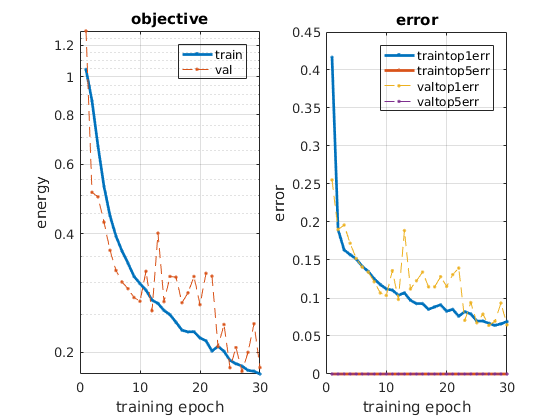
\includegraphics[scale=0.8]{init_1.png}
		\caption{network 1 training}
		\label{fig:training1}
	\end{center}
\end{figure}

\begin{figure}[h]
	\begin{center}
		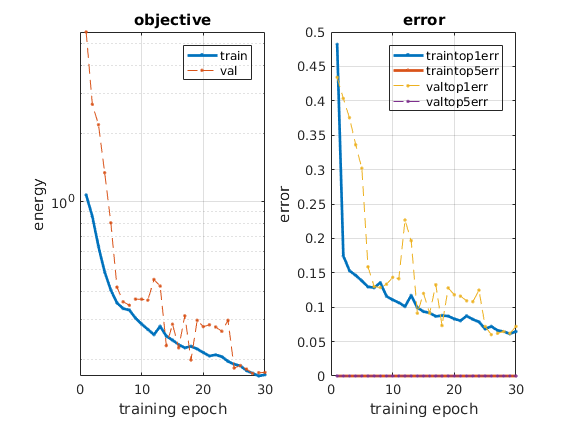
\includegraphics[scale=0.8]{init_2.png}
		\caption{network 2 training}
		\label{fig:training1}
	\end{center}
\end{figure}

\begin{figure}[h]
	\begin{center}
		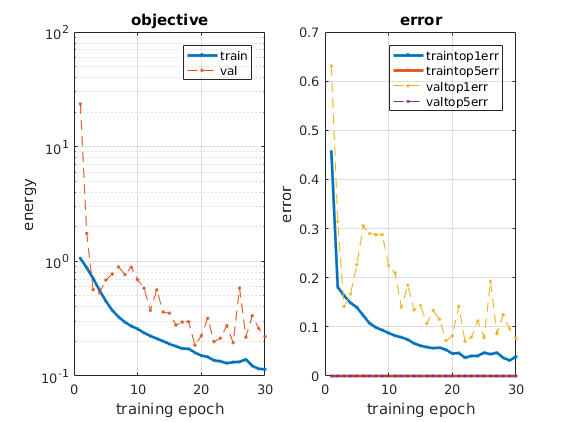
\includegraphics[scale=0.8]{init_3.png}
		\caption{network 3 training}
		\label{fig:training1}
	\end{center}
\end{figure}

\begin{figure}[h]
	\begin{center}
		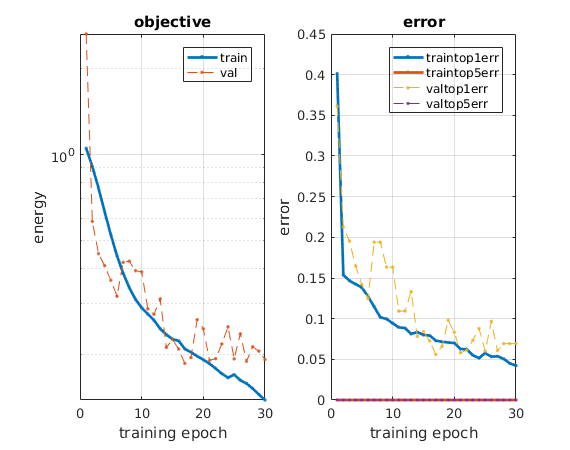
\includegraphics[scale=0.8]{init_4.png}
		\caption{network 4 training}
		\label{fig:training1}
	\end{center}
\end{figure}

\begin{figure}[h]
	\begin{center}
		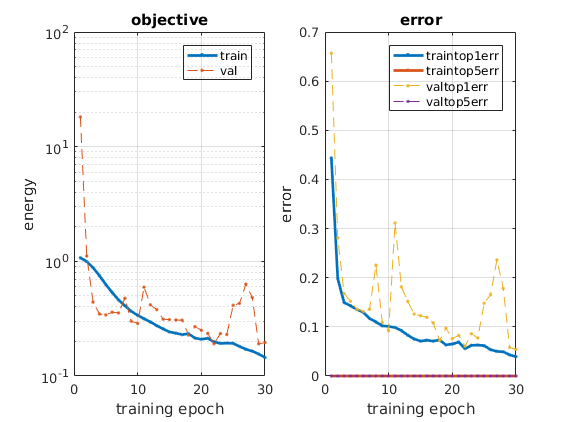
\includegraphics[scale=0.8]{init_5.png}
		\caption{network 5 training}
		\label{fig:training5}
	\end{center}
\end{figure}

\begin{figure}[h]
	\begin{center}
		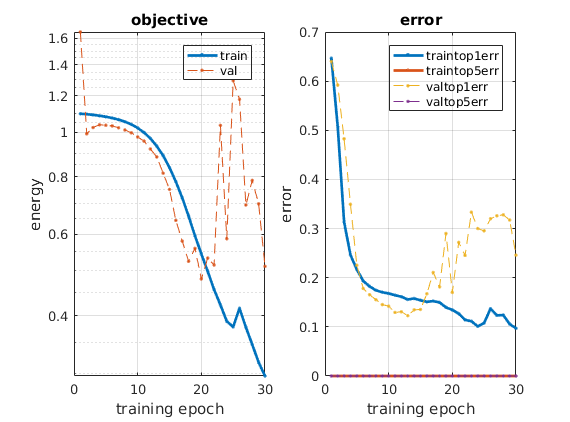
\includegraphics[scale=0.8]{init_6.png}
		\caption{network 6 training}
		\label{fig:training6}
	\end{center}
\end{figure}

\chapter{Evaluate the network}

\section{Compute the accuracy of each network}

Here is the code that I used in order to compute the accuracy of the network. It evalutates a training set that is composed, in order, of:
\begin{enumerate}
\item 500 crop patches
\item 500 weed patches
\item 500 ground patches
\end{enumerate}

\begin{lstlisting}
clear

% load the pre-trained CNN
net = cnn_cwfid();

testingDir = fullfile(vl_rootnn, 'data', 'cwfid','testing');
testingCropDir = fullfile(testingDir,'crop');
testingWeedDir = fullfile(testingDir,'weed');
testingGroundDir = fullfile(testingDir,'ground');

%only the second half of the test images are using 
%because the first half is for validation
%get testing crop images 
listing = dir(testingCropDir);
listing=listing(~ismember({listing.name},{'.','..','Thumbs.db'}));
for i=1 : (size(listing,1) - 500)
    cropImTesting(:,:,:,i)=imread(fullfile(testingCropDir,listing(i+500).name));
end

%get testing weed images 
listing = dir(testingWeedDir);
listing=listing(~ismember({listing.name},{'.','..','Thumbs.db'}));
for i=1 : (size(listing,1) - 500)
    weedImTesting(:,:,:,i)=imread(fullfile(testingWeedDir,listing(i+500).name));
end

%get testing ground images 
listing = dir(testingGroundDir);
listing=listing(~ismember({listing.name},{'.','..','Thumbs.db'}));
for i=1 : (size(listing,1) - 500)
    groundImTesting(:,:,:,i)=imread(fullfile(testingGroundDir,listing(i+500).name));
end

%put the testing image all together
data = single(reshape(cat(4,cropImTesting,weedImTesting,groundImTesting),51,51,3,[]));

%remove last layer: softmax  
net.layers{end}.type = 'softmax';

% run the CNN
res = vl_simplenn(net, data);

% get the classification result
scores = squeeze(gather(res(end).x)) ;
[bestScore, best] = max(scores) ;

%calculate accuracy
error = 0;
i = 1;
for j= 1:500
    if best(j) ~= i
        error= error+1;
    end
end

%accuracy Crop
accuracyCrop = 1-error/500;

error = 0;
i = 2;
for j= 501:1000
    if best(j) ~= i
        error= error+1;
    end
end

%accuracy weed
accuracyWeed = 1-error/500;

error = 0;
i = 3;
for j= 1001:1500
    if best(j) ~= i
        error= error+1;
    end
end

%accuracy ground
accuracyGround = 1-error/500;

%global accuracy of the network
accuracy = (accuracyCrop+accuracyWeed+accuracyGround)/3;

\end{lstlisting}

With this code for the 6 networks we have these results:

\begin{table}[h]
\centering

\begin{tabular}{|c|c|c|c|c|}
 \hline
 \textbf{Network} & \textbf{Accuracy} & \textbf{Accuracy Crop} & \textbf{Accuracy Ground} & \textbf{Accuracy Weed} \\ \hline
 1 & 94,00\% & 92,80\%  & 99,80\%  & 89,40\%  \\ \hline
 2 & 94,07\% & 95,60\%  & 99,80\%  & 86,80\%  \\ \hline
 3 & 92,53\% & 92,20\%  & 99,80\%  & 85,60\%  \\ \hline
 4 & 94,13\% & 93,00\%  & 99,80\%  & 89,60\%  \\ \hline
 \textbf{5} & \textbf{94,20\%} & \textbf{94,00\%}  & \textbf{99,80\%}  & \textbf{88,80\%}  \\ \hline
 6 & 92,33\% & 93,60\%  & 99,80\%  & 83,60\%  \\ \hline
\end{tabular}
\end{table}

\begin{figure}[h]
	\begin{center}
		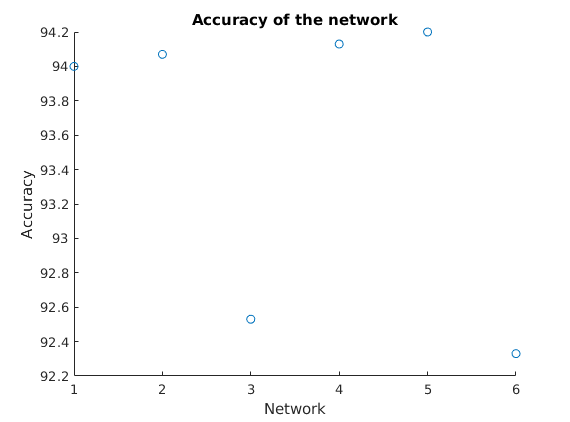
\includegraphics[scale=0.6]{accuracy.png}
		\caption{accuracy of the networks}
		\label{fig:accuracyNetworks}
	\end{center}
\end{figure}

The network that has the highest accuracy is network 5. From now on I will discuss and talk about network 5 only because it has the best performance. 

\section{Changing the number of maps of each convolutional filter}

Once the network has been selected I tried to change the number of maps of each convolutional filter in order to increase the accuracy. Here are some combination of number of maps that I used and the correspondent accuracy.

\begin{table} [h]
\begin{center}
\begin{tabular}{|c|c|c|c|c|}
 \hline
 \textbf{Filter 1} & \textbf{Filter 2} & \textbf{Filter 3} & \textbf{Filter 4} & \textbf{Accuracy} \\ \hline
 10 & 20 & 40  & 80  & 94,20\%  \\ \hline
 15 & 30 & 60  & 120  & 92,60\%  \\ \hline
 \textbf{8} & \textbf{16} & \textbf{32}  & \textbf{64}  & \textbf{94,33\%}  \\ \hline
 7 & 14 & 28  & 56  & 93,73\%  \\ \hline
 9 & 18 & 36  & 72  & 93,20\%  \\ \hline
 12 & 24 & 48  & 96  & 92,53\%  \\ \hline
 
\end{tabular}
\end{center} 
\end{table}
  
\begin{figure}[h]
	\begin{center}
		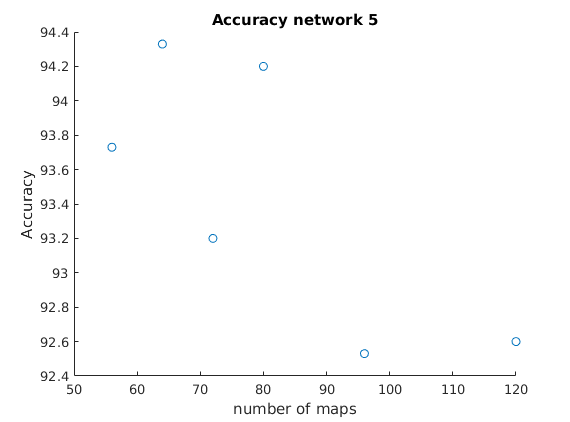
\includegraphics[scale=0.6]{maps_accuracy.png}
		\caption{accuracy VS number of maps; only the number of maps of the last filter layer is plotted in the 					 graph}
		\label{fig:accuracyMaps}
	\end{center}
\end{figure}

\newpage   
This is the training graph with a better combination of number of maps. This configuration is the final one that I used for the given assignment and has a global accuracy of \textbf{94,33\%} \textbf{94,20\%} for crop \textbf{99,80\%} for ground and \textbf{89,00\%} for weed.

\begin{figure}[h]
	\begin{center}
		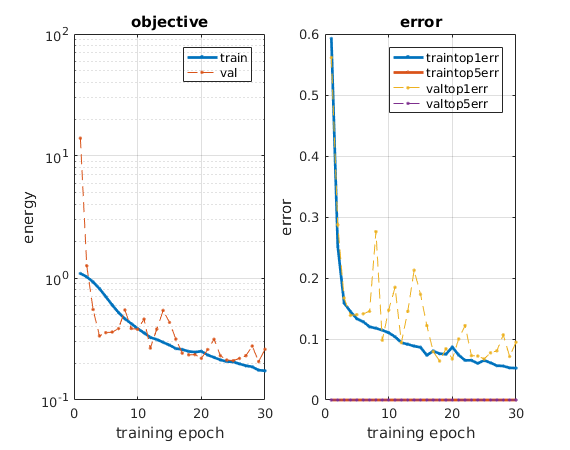
\includegraphics[scale=0.6]{final.png}
		\caption{final training}
		\label{fig:FinalTraining}
	\end{center}
\end{figure}

\newpage
\section{Sliding window approach}

In order to have a rough segmentation of the training set I also used to evaluate the network the sliding window approach. The code below shows how the approach was implemented. It use a stride of 10 and calculate for each image test the accuracy and the confusion matrix. The ground truth that I used to calculate these metrics was included into the CWFID dataset.  

\begin{lstlisting}

close all
clear
clc

%define the size of the patches
dim = 51;
%define the stride of the sliding window
stride = 10;
%crop = 1, weed = 2, ground = 3
crop = 1;
weed = 2;
ground = 3;

% load the pre-trained CNN
net = cnn_cwfid();
%remove last layer: softmax  
net.layers{end}.type = 'softmax';
net.mode = 'test';

testingDir = fullfile(vl_rootnn, 'data', 'cwfid','testing');
testingSlidingWindowDir = fullfile(testingDir,'sliding window');
annotationDir = fullfile(testingDir,'annotation');

listing = dir(testingSlidingWindowDir);
listing=listing(~ismember({listing.name},{'.','..','Thumbs.db'}));
%get the testing image
for i=1 : size(listing,1)
    slidingWindowImTesting(:,:,:,i)=imread(fullfile(testingSlidingWindowDir,listing(i).name));
end

listing = dir(annotationDir);
listing=listing(~ismember({listing.name},{'.','..','Thumbs.db'}));
%get the annotation image
for i=1 : size(listing,1)
    AnnotationIm(:,:,:,i)=imread(fullfile(annotationDir,listing(i).name));
end

%for all the images
for i=1 : size(slidingWindowImTesting,4)
    cont1 = 1;
    for j=1 : stride : (size(slidingWindowImTesting,2)-dim)
       for k=1 : stride : (size(slidingWindowImTesting,1)-dim)
           %get the patches
           im(:,:,:,cont1) = single(imcrop(slidingWindowImTesting(:,:,:,i),...
               [j,k,dim-1,dim-1]));
           cont1 = cont1+1;
       end
    end
    
   %subtract the data mean 
   dataMean = mean(im(:,:,:),3);
   im = bsxfun(@minus, im, dataMean) ;
   %evaluates the patches    
   res = vl_simplenn(net, im);
   scores = squeeze(gather(res(end).x)) ;
   [bestScore, best] = max(scores) ;

   I = reshape(best,int16((size(slidingWindowImTesting,1)-dim)/stride),...
        int16((size(slidingWindowImTesting,2)-dim)/stride));
   Icrop = reshape(scores(crop,:),int16((size(slidingWindowImTesting,1)-dim)/stride),...
        int16((size(slidingWindowImTesting,2)-dim)/stride));
   Icrop = imresize(Icrop,[size(slidingWindowImTesting,1),size(slidingWindowImTesting,2)]);
   Iweed = reshape(scores(weed,:),int16((size(slidingWindowImTesting,1)-dim)/stride),...
        int16((size(slidingWindowImTesting,2)-dim)/stride));
   Iweed = imresize(Iweed,[size(slidingWindowImTesting,1),size(slidingWindowImTesting,2)]);
   Iground = reshape(scores(ground,:),int16((size(slidingWindowImTesting,1)-dim)/stride),...
        int16((size(slidingWindowImTesting,2)-dim)/stride));
   Iground = imresize(Iground,[size(slidingWindowImTesting,1),size(slidingWindowImTesting,2)]); 
   
   %create an image with the best class with color: crop=green weed=red
   %ground=black
   for s=1 : size(I,1)
        for v=1 : size(I,2)
            if I(s,v) == crop
               Im((s-1)*stride+1:s*stride,(v-1)*stride+1:v*stride,1) = 0;
               Im((s-1)*stride+1:s*stride,(v-1)*stride+1:v*stride,2) = 255;
               Im((s-1)*stride+1:s*stride,(v-1)*stride+1:v*stride,3) = 0;
            end
            if I(s,v) == weed
               Im((s-1)*stride+1:s*stride,(v-1)*stride+1:v*stride,1) = 255;
               Im((s-1)*stride+1:s*stride,(v-1)*stride+1:v*stride,2) = 0; 
               Im((s-1)*stride+1:s*stride,(v-1)*stride+1:v*stride,3) = 0;
            end
            if I(s,v) == ground
               Im((s-1)*stride+1:s*stride,(v-1)*stride+1:v*stride,1) = 0;
               Im((s-1)*stride+1:s*stride,(v-1)*stride+1:v*stride,2) = 0;
               Im((s-1)*stride+1:s*stride,(v-1)*stride+1:v*stride,3) = 0;
            end
        end
   end
   
   figure
   subplot(3,2,1)
   imshow(slidingWindowImTesting(:,:,:,i));
   title('original')
   subplot(3,2,2)
   imshow(AnnotationIm(:,:,:,i));
   title('annotation')
   subplot(3,2,3)
   imshow(Im)
   title('best')
   subplot(3,2,4)
   imagesc(Icrop),colorbar
   title('crop')
   subplot(3,2,5)
   imagesc(Iweed),colorbar
   title('weed')
   subplot(3,2,6)
   imagesc(Iground),colorbar
   title('ground')
   
   %get the label from annotation and the predicted class
   cont = 0;
   for s = 1 : size(Im,1)
       for v = 1 : size(Im,2)
           cont= cont+1;
           if AnnotationIm(s,v,1,i) == 255
               label(cont)= weed;
           else if AnnotationIm(s,v,2,i) == 255
                    label(cont)= crop;
                else 
                label(cont)= ground;
               end
           end
           if Im(s,v,1) == 255
               predicted(cont)= weed;
           else if Im(s,v,2) == 255
                  predicted(cont)= crop;
                else
                predicted(cont)= ground;
               end
           end
       end
   end
   
   %calculate confusion matrix
   C = confusionmat(label,predicted);
   Accuracy = (C(1,1)+C(2,2)+C(3,3))/(C(1,1)+C(1,2)+C(1,3)+C(2,1)+C(2,2)...
       +C(2,3)+C(3,1)+C(3,2)+C(3,3));
   
end

\end{lstlisting}


\chapter{Summary and future extensions}

\chapter{Appendix}

\section{Reference document}
 \begin{itemize}
 
 	\item\url{http://rd.springer.com/chapter/10.1007%2F978-3-319-16220-1_8}
	
 \end{itemize}

\section{Software and tool used}

\begin{itemize}
	
	\item LaTeX (\url{http://www.latex-project.org/}) : to redact and to format this document
	
	\item Matlab R2016a (\url{http://uk.mathworks.com/products/matlab/}) : to compute and 					  evaluate the network
	
	\item MatConvNet (\url{http://www.vlfeat.org/matconvnet/}) : MATLAB toolbox implementing 				  Convolutional Neural Networks (CNNs) 
	 
\end{itemize}

\end{document}          
